\title{A real-time state estimation for an electric race car}
\author{Dominik Stiller}
\date{June 8, 2020}

\documentclass[numbers=noenddot]{scrreprt}


%----------------------------------------------------------------------------
% Package Includes
%----------------------------------------------------------------------------
\usepackage[USenglish]{babel}
\usepackage[T1]{fontenc}
\usepackage[utf8]{inputenc}
\usepackage{lmodern}

%\usepackage{showframe}
\usepackage{tocloft}
\usepackage{chngcntr}
\usepackage{amsmath}
\usepackage{mathtools}
\usepackage{mathbbol}
\usepackage{interval}
\usepackage{graphicx}
\usepackage{subcaption}
\usepackage[hidelinks]{hyperref}
\usepackage{geometry}
\usepackage{textcomp}
\usepackage{pifont}
\usepackage{siunitx}
\usepackage{setspace}
\usepackage{array}
\usepackage[outputdir=build]{minted}
\usepackage[toc,page]{appendix}
\usepackage{tabularx}
\usepackage{colortbl}
\usepackage{makecell}
\usepackage{csquotes}
\usepackage{xcolor}
\usepackage[bottom,hang,flushmargin]{footmisc}
\usepackage[toc,nonumberlist,acronym,nopostdot]{glossaries}
\usepackage[intoc]{nomencl}
\usepackage{etoolbox}
\usepackage[
	backend=biber,
	bibwarn=true,
	bibencoding=utf8,
	sortlocale=en_US,
	%url=false,
	style=ieee
]{biblatex}
\usepackage[activate={true,nocompatibility},final,tracking=true,kerning=true,spacing=true,factor=1100,stretch=10,shrink=10]{microtype}


%----------------------------------------------------------------------------
% Package Config
%----------------------------------------------------------------------------

% KOMA-Script
\KOMAoptions{
	pagesize=pdftex,
	twoside=false,		% Einseitiger Druck.
	parskip=half,		% Halbe Zeile Abstand zwischen Absätzen.
	headheight = 12pt,	% Höhe der Kopfzeile
	headsepline,		% Linie nach Kopfzeile.
	footsepline,		% Linie vor Fusszeile.
	footheight = 16pt,	% Höhe der Fusszeile
	abstract=true,		% Abstract Überschriften
	DIV=calc,			% Satzspiegel berechnen
	headinclude=false,	% Kopfzeile nicht in den Satzspiegel einbeziehen
	footinclude=false,	% Fußzeile nicht in den Satzspiegel einbeziehen
	listof=totoc,		% Abbildungs-/ Tabellenverzeichnis im Inhaltsverzeichnis darstellen
	toc=bibliography	% Literaturverzeichnis im Inhaltsverzeichnis darstellen
}
\clubpenalty = 10000 % schließt Seitenumbruch nach der ersten Zeile eines neuen Absatzes aus
\widowpenalty = 10000 % schließt die letzte Zeile eines Absatzes steht auf einer neuen Seite aus
\displaywidowpenalty=10000
\renewcommand{\topfraction}{.75}

% graphicx
\graphicspath{ {./images/} }

% biblatex
\addbibresource{./misc/references.bib}

% Microtype
% http://www.khirevich.com/latex/microtype/
\SetProtrusion{encoding={*},family={bch},series={*},size={6,7}}
			     {1={ ,750},2={ ,500},3={ ,500},4={ ,500},5={ ,500},
	             6={ ,500},7={ ,600},8={ ,500},9={ ,500},0={ ,500}}
\SetExtraKerning[unit=space]
   				{encoding={*}, family={bch}, series={*}, size={notesize,small,normalsize}}
				{\textendash={400,400}, % en-dash, add more space around it
	               "28={ ,150}, % left bracket, add space from right
	               "29={150, }, % right bracket, add space from left
					\textquotedblleft={ ,150}, % left quotation mark, space from right
					\textquotedblright={150, }} % right quotation mark, space from left
\SetExtraKerning[unit=space]
				{encoding={*}, family={qhv}, series={b}, size={large,Large}}
				{1={-200,-200}, \textendash={400,400}}
\SetTracking{encoding={*}, shape=sc}{40}
\microtypecontext{spacing=nonfrench}

% glossary
\renewcommand*{\glsgroupskip}{}

% chngcntr
\counterwithout{figure}{chapter}
\counterwithout{table}{chapter}
\counterwithout{equation}{chapter}

% minted
\usemintedstyle{friendly}
\newminted{python}{
	mathescape,
	linenos,
	numbersep=5pt,
	frame=lines,
	framesep=2mm
}
\newmintinline{python}{}

% amsmath
\DeclareMathOperator*{\argmax}{arg\,max}
% https://tex.stackexchange.com/a/43009
\DeclarePairedDelimiter\abs{\lvert}{\rvert}
\DeclarePairedDelimiter\norm{\lVert}{\rVert}
\makeatletter
\let\oldabs\abs
\def\abs{\@ifstar{\oldabs}{\oldabs*}}
\let\oldnorm\norm
\def\norm{\@ifstar{\oldnorm}{\oldnorm*}}
\makeatother

% xcolor
\definecolor{hpe-green}{HTML}{01A982}
\definecolor{hpe-orange}{HTML}{FF8300}

% nomencl
\renewcommand{\nomname}{List of Symbols}
\newcommand{\nomunit}[1]{\renewcommand{\nomentryend}{\hspace*{\fill}\si{#1}}}
\renewcommand\nomgroup[1]{%
  \item[\bfseries
  \ifstrequal{#1}{P}{Physics Constants}{%
  \ifstrequal{#1}{N}{Number Sets}{%
  \ifstrequal{#1}{O}{Other Symbols}{}}}%
]}
\makenomenclature

% Enable ligatures in pdf figures
%\pdfinclusioncopyfonts=1

% pifont
\newcommand{\xmark}{\ding{53}}%


%----------------------------------------------------------------------------
% Styling
%----------------------------------------------------------------------------

% Page
\geometry{margin=2.5cm, foot=1cm, bindingoffset=0mm}%bindingoffset=8mm

% 
\KOMAoptions{fontsize=12pt}
\DeclareMathSizes{12pt}{12pt}{10pt}{10pt}
\setkomafont{title}{\Huge\textbf}
\onehalfspacing

% Table of Contents
\setcounter{tocdepth}{1}

\renewcommand{\appendixname}{Appendix}


%----------------------------------------------------------------------------
% Custom Commands
%----------------------------------------------------------------------------

\newcommand*{\vcenteredhboxleft}[1]{
	\raggedright
	\begingroup
	\setbox0=\hbox{#1}\parbox{\wd0}{\box0}
	\endgroup
}

\newcommand*{\vcenteredhboxright}[1]{
	\raggedleft
	\begingroup
	\setbox0=\hbox{#1}\parbox{\wd0}{\box0}
	\endgroup
}

\newcommand{\multilinecell}[2][c]{%
	\begin{tabular}
		[#1]{@{}l@{}}#2
	\end{tabular}
}

\newcommand\todo[1]{\textcolor{orange}{#1}}


\makeglossaries
\newglossaryentry{perfcomp}{
	name={performance components},
	description={the collective term for \gls{tv} and \gls{tc}, the components of the \gls{vdc} which maximize the vehicle's performance}
}

\newacronym{vdc}{VDC}{vehicle dynamics control}
\newacronym{ekf}{EKF}{extended Kalman filter}
\newacronym{cog}{CG}{center of gravity}
\newacronym{gnss}{GNSS}{global navigation satellite system}
\newacronym{gps}{GPS}{Global Positioning System}


\begin{document}
	\pagenumbering{Roman}
	\pagestyle{empty}
	\makeatletter
	\begin{titlepage}
		\vcenteredhboxleft{
\includegraphics[height=1.8cm]{logo_engineering.pdf}}
\hfill
\vcenteredhboxright{
\includegraphics[height=2cm]{logo_dhbw.pdf}}

\vfill
\begin{center}
	\rule{\textwidth}{1pt}
	{
		\Huge
		\bfseries
		A real-time state estimation \\ for an electric race car
		\par
	}
	\vspace{-0.2cm} 
	\rule{\textwidth}{1pt}

	\vfill

	\textsc{Research Project / T3100}
	
	\vfill

	for the study program \\ \textbf{Computer Science}
	
	at the \\ \textbf{Baden-Wuerttemberg Cooperative State University Stuttgart}
	
	by \\ \textbf{\@author}
\end{center}

\vfill

\begin{tabbing}
	mmmmmmmmmmmmmmmmmmmmmmmmmm				\= \kill
	\textbf{Submission Date}				\> \@date \\
	\textbf{Thesis Supervisor}           	\> Marco Busch \\
	\textbf{University Supervisor}          \> Prof. Dr. Zoltán Ádam Zomotor \\
	\textbf{Matriculation Number, Course}  	\> 4369179, TINF17A
\end{tabbing}

	\end{titlepage}
	
	\section*{Declaration of Authorship}
	I hereby declare that the thesis submitted with the title \textit{\@title} is my own unaided work. All direct or indirect sources used are acknowledged as references.

Neither this nor a similar work has been presented to an examination committee or published.

\vspace{4em}

Sindelfingen
\hspace{1.3cm}
June 8, 2020
\vspace{-0.4cm}
\\
\rule{15cm}{0.4pt}\\
Place
\hspace{2.5cm}
Date
\hspace{4.5cm}
\@author
	\makeatother
	\vfill
	
	\section*{Confidentiality Clause}
	This thesis contains confidential data of \textit{DHBW Engineering Stuttgart e.V.} This work may only be made available to the university supervisor. Any publication and duplication of this thesis--even in part--is prohibited.

An inspection of this work by third parties requires the expressed permission of the author and \textit{DHBW Engineering Stuttgart e.V.} 
	\vfill

	\begin{abstract}
		Real-time computer vision applications with deep learning-based inference require hardware-specific optimization to meet stringent performance requirements. Frameworks have been developed to generate the optimal low-level implementation for a certain target device based on a high-level input model using machine learning in a process called autotuning. However, current implementations suffer from inherent resource utilization inefficiency and bad scalability which prohibits large-scale use.

In this paper, we develop a load-aware scheduler which enables large-scale autotuning. The scheduler controls multiple, parallel autotuning jobs on shared resources such as CPUs and GPUs by interleaving computations, which minimizes resource idle time and job interference. The scheduler is a key component in our proposed Autotuning as a Service reference architecture to democratize autotuning. Our evaluation shows good results for the resulting inference performance and resource efficiency.
	\end{abstract}

	\setlength{\cftbeforetoctitleskip}{2.1em}
	\begin{spacing}{1.15}
	   \tableofcontents
	\end{spacing}
	\clearpage
	\thispagestyle{empty}
	
	\pagestyle{plain}
	
	%----------------------------------------------------------------------------
	% Preface
	%----------------------------------------------------------------------------
	\printacronyms
	\clearpage
	
	\addcontentsline{toc}{chapter}{\listfigurename}
	\listoffigures
	\clearpage
	\addcontentsline{toc}{chapter}{\listtablename}
	\listoftables
	\renewcommand\listoflistingscaption{List of Source Codes}
	\listoflistings
	\clearpage
	
	\pagenumbering{arabic}
	
	\pagestyle{headings}
	
	\addtocontents{toc}{\protect\thispagestyle{empty}}
	\obeylines
	%----------------------------------------------------------------------------
	% Content
	%----------------------------------------------------------------------------
	\chapter{Introduction}
	FS + esleek

Problem + motivation, why gppd SE is important

Scope, what will be covered
	\chapter{Background}
	The state estimation of a vehicle sits at the intersection of vehicle dynamics and control theory. Both knowledge of the dynamics of a race car and the algorithms to model their physics in equations and software is required to design a successful solution. Therefore, we explore the fundamentals of vehicle dynamics, estimation algorithms and sensor failure detection in this chapter.

Throughout this thesis, the conventions of ISO 8855~\cite{ISO.2011} will be used, which assumes a right-handed coordinate system. The vehicle coordinate system uses an upward $z$-axis with a forward $x$-axis and a leftward $y$-axis, while the earth-fixed coordinate system uses an upward $z$-axis with an eastward $x$-axis and a northward $y$-axis. The vehicle's\gls{cog} is used as origin/reference point of the vehicle coordinate system. In case of mixed coordinate systems, left-superscript will be used to denote the reference frame (e.g., $\prescript{V}{}{x}$ for vehicle coordinates, $\prescript{E}{}{x}$ for earth-fixed coordinates).



\section{Rigid Body Kinematics}
The fundamental laws of mechanics apply to race cars as they do to any other body. These laws relate, among others, the body's linear and angular position and its time derivatives, resulting in translational and rotational changes. Their three-dimensional vector definitions are shown in equations \ref{eq:linear-quantities} and \ref{eq:angular-quantities}. To simplify the equations, a rigid body is assumed. This means, that deformations which occur in the vehicle during dynamic maneuvers are negligibly small or vanish. Therefore, points on the body maintain the same distance relative to each other at all times. Furthermore, a two-dimensional motion in the road plane can be assumed in many cases because the effects vertical dynamics are negligible. The simplified equations for that case will also be shown.

\begin{subequations}\label{eq:linear-quantities}
\begin{alignat}{2}%
p &= \begin{bmatrix}x, y, z\end{bmatrix}^T \\%
v &= \begin{bmatrix}v_x, v_y, v_z\end{bmatrix}^T \\%
a &= \begin{bmatrix}a_x, a_y, a_z\end{bmatrix}^T%
\end{alignat}
\end{subequations}
\begin{subequations}\label{eq:angular-quantities}
\begin{alignat}{2}%
\varphi &= \begin{bmatrix}\phi, \theta, \psi\end{bmatrix}^T \\%
\omega &= \begin{bmatrix}\dot{\phi}, \dot{\theta}, \dot{\psi}\end{bmatrix}^T \\%
\alpha &= \begin{bmatrix}\ddot{\phi}, \ddot{\theta}, \ddot{\psi}\end{bmatrix}^T%
\end{alignat}
\end{subequations}

The linear displacement $p$ of a body describes its position relative to the origin of its reference frame. It comprises a longitudinal component along the $x$-axis, a lateral component along the $y$-axis and a vertical component along the $z$-axis. Its first time derivative $v = \frac{dr}{dt}$ and second time derivative $a = \frac{d^2r}{dt^2}$ are the body's linear velocity and acceleration, respectively. \\ The angular orientation $\varphi$ of a body describes its rotation in the reference frame. It can be described by the roll angle $\phi$ around the $x$-axis, the pitch angle $\theta$ around the $y$-axis and the yaw angle $\psi$ around the $z$-axis. The angular velocity $\omega$ and acceleration $\alpha$ describe the element-wise time derivatives of these angles.


\subsection{Transformation of Linear Velocities}
All points on a rigid body experience the same angular velocity, i.e. $\omega^A = \omega^B$ for any two points $A, B$ on that body at all times. However, these two points will generally not have the same linear velocity vector, since it is affected by their location $r$ relative to the \gls{cog}. Only when $\omega = \mathbb{0}$, the linear velocity is equal for all points on the body, i.e. $v^A = v^B$. If there is a non-zero angular velocity, equation \ref{eq:offcenter-velocity-3d} holds for any point $P$, assuming the velocity at the \gls{cog} is known (the expanded form can be found in Appendix \ref{sec:appendix-transformation-linvel}).

% For SFII transformation
\begin{equation}\label{eq:offcenter-velocity-3d}%
v^P = v^{CG} + \omega \times r^P%
\end{equation}

This becomes easier to visualize when regarding the two-dimensional case, where $v_z$, $\dot{\phi}$ and $\dot{\theta}$ are disregarded, as shown in equation \ref{eq:offcenter-velocity-2d}.

\begin{equation}\label{eq:offcenter-velocity-2d}%
v^P%
= \begin{bmatrix}v_x^{CG} \\ v_y^{CG} \\ 0\end{bmatrix} + \begin{bmatrix}0 \\ 0 \\ \dot{\psi}\end{bmatrix} \times \begin{bmatrix}r_x \\ r_y \\ r_z\end{bmatrix}%
= \begin{bmatrix}v_x^{CG} \\ v_y^{CG} \\ 0\end{bmatrix} + \begin{bmatrix}-\dot{\psi} \cdot r_y \\ \dot{\psi} \cdot r_x \\ 0\end{bmatrix}%
 \end{equation}

Let us regard the example scenario shown in figure \ref{fig:offcenter-velocity}, where the vehicle has a positive yaw rate and the \gls{cog} is moving forward and to the left. Point $A$ is at the front left ($r_x > 0$, $r_y > 0$), while point $B$ is at the rear right ($r_x < 0$, $r_y < 0$). Since $r$ is defined relative to the \gls{cog}, its position is $\mathbb{0}$. Due to the positive yaw rate, $A$ experiences a higher $v_y$ but lower $v_x$ than the \gls{cog}. $B$, on the other hand, experiences a higher $v_x$ but lower $v_y$ than the \gls{cog}. If the yaw rate were zero, all points would experience the same linear velocity.

\begin{figure}
	\centering
	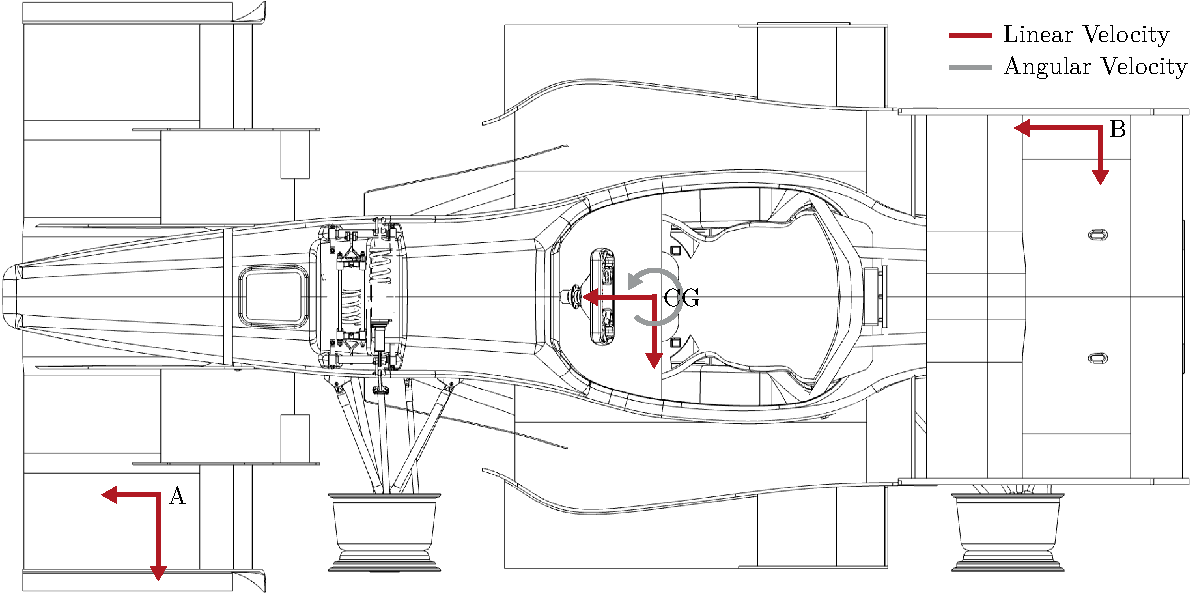
\includegraphics[width=\textwidth]{offcenter_velocity}%
	\caption{Experienced velocities at off-center points}
	\label{fig:offcenter-velocity}
\end{figure}


\subsection{Transformation of Linear Accelerations}
Like the angular velocity, the angular acceleration is the same at every point on a rigid body, i.e. $\alpha^A = \alpha^B$ for any two points $A, B$ on that body. However, these two points will generally not experience the same linear acceleration. Only if the rotational motion components $\omega$ and $\alpha$ are $\mathbb{0}$, the linear acceleration is equal for all points on the body, i.e. $a^A = a^B$. In the general case, equation \ref{eq:offcenter-acceleration-3d} holds for any point $P$ at location $r$ (the expanded form can be found in Appendix \ref{sec:appendix-transformation-linacc}).

\begin{equation}\label{eq:offcenter-acceleration-3d}%
a^P = a^{CG} + \alpha \times r^P + \omega \times (\omega \times r^P)%
\end{equation}

We can identify two additional components which affect the experienced linear acceleration. The term $\alpha \times r$ is the tangential acceleration along the circular path around the center of rotation, which is $a_{tan} = \alpha \cdot r$ in scalar notation. More significant due to the squared angular velocity, however, is the introduction of the centripetal acceleration $a_c$ in the term $\omega \times (\omega \times r)$. This term is the vector-equivalent of the acceleration resulting from the centripetal force $F_c$ in equation \ref{eq:centripetal-acceleration}.

\begin{equation}\label{eq:centripetal-acceleration}%
F_c = \frac{mv^2}{r} \iff a_c = \frac{v^2}{r} = \omega^2 r%
\end{equation}

The two-dimensional form, shown in equation \ref{eq:offcenter-acceleration-2d}, is more intuitive than its three-dimensional counterpart. Here, $a_z$, $\dot{\phi}$, $\dot{\theta}$, $\ddot{\phi}$ and $\ddot{\theta}$ are assumed to be zero. The inward-direction of the centripetal effect can be seen by the negative signs of the angular velocity part.

\begin{equation}\label{eq:offcenter-acceleration-2d}%
a^P%
= \begin{bmatrix}a_x^{CG} \\ a_y^{CG} \\ 0\end{bmatrix}%
+ \begin{bmatrix}0 \\0 \\ \ddot{\psi}\end{bmatrix} \times \begin{bmatrix}r_x \\ r_y \\ r_z\end{bmatrix} \\%
+ \begin{bmatrix}0 \\ 0 \\ \dot{\psi}\end{bmatrix} \times \left(\begin{bmatrix}0 \\ 0 \\ \dot{\psi}\end{bmatrix} \times \begin{bmatrix}r_x \\ r_y \\ r_z\end{bmatrix}\right)%
= \begin{bmatrix}a_x^{CG} \\ a_y^{CG} \\ 0\end{bmatrix}%
+ \begin{bmatrix}-\ddot{\psi} \cdot r_y \\ \ddot{\psi} \cdot r_x \\ 0\end{bmatrix}%
+ \begin{bmatrix}-\dot{\psi}^2 \cdot r_x \\ -\dot{\psi}^2 \cdot r_y \\ 0\end{bmatrix}%
\end{equation}

We demonstrate these effects in the example scenario shown in figure \ref{fig:offcenter-acceleration}, which is similar to the one in the previous subsection, but with an additional positive yaw acceleration. In point $A$, the tangential and centripetal acceleration cancel out and even surpass the linear acceleration experienced in the \gls{cog}, resulting in a negative $a_x$ and a much lower $a_y$. The opposite effect occurs in point $B$, where both $a_x$ and $a_y$ are amplified.

\begin{figure}
	\centering
	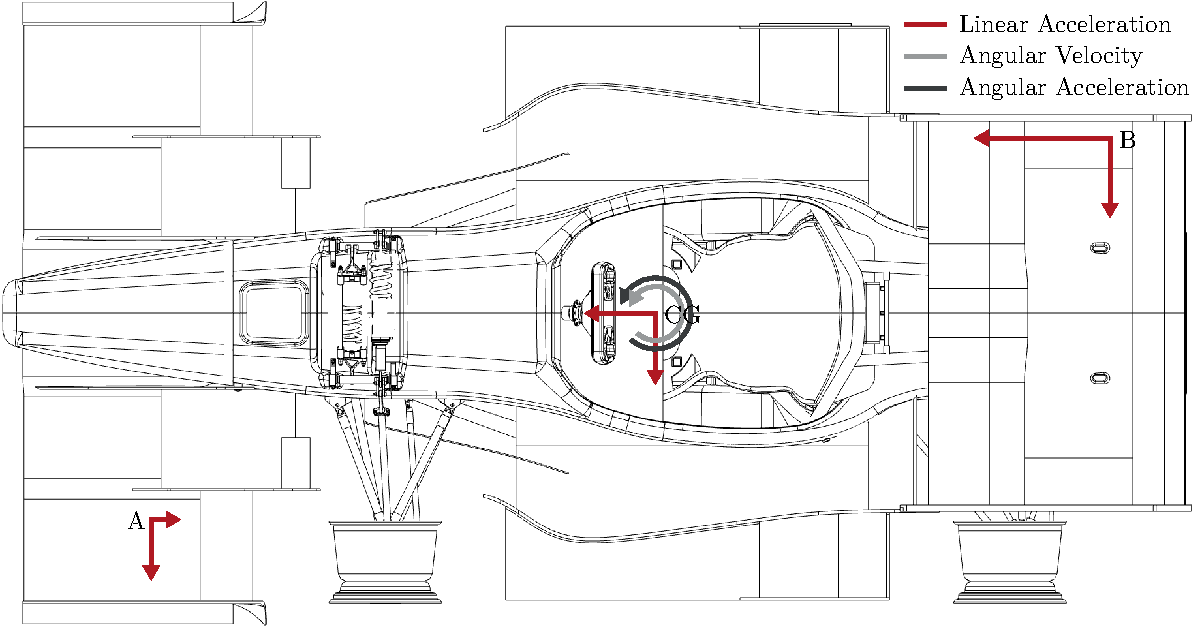
\includegraphics[width=\textwidth]{offcenter_acceleration}%
	\caption{Experienced acceleration at off-center points}
	\label{fig:offcenter-acceleration}
\end{figure}


\subsection{Calculate Angular Acceleration from Linear Acceleration}
Direct measurement of the angular acceleration is often not possible. However, individual components of $\alpha$ can be calculated with two known linear acceleration vectors from different points $A, B$ with known locations $r^A, r^B$ using equation \ref{eq:angacc-from-linacc-3d}. It is derived from equation \ref{eq:offcenter-acceleration-3d}, with $\Delta a = a^A - a^B$, $\Delta r = r^A - r^B$ and $a^{CG}$ being eliminated by the difference. The points must not be on the rotation axis of the calculated component of $\alpha$, otherwise they experience no angular acceleration. Thus, at least three non-collinear points are required to determine all components of $\alpha$. While the inverse of a cross product is not uniquely determined as can be seen by the scalar factor $t$, $t = 0$ works well in practice.

\begin{equation}\label{eq:angacc-from-linacc-3d}%
\Delta a = \alpha \times \Delta r + \omega \times (\omega \times \Delta r) \implies%
\alpha = \frac{\Delta r \times (\Delta a - \omega \times (\omega \times \Delta r))}{\norm{\Delta r}^2} + t \cdot \Delta r, t \in \mathbb{R}%
\end{equation}

In two dimensions, this becomes easier to understand. Calculation of the yaw acceleration from the longitudinal and lateral accelerations of two points is shown in equation \ref{eq:angacc-from-linacc-2d}. We can see that the accelerations and distances from different axes are cross-correlated. The equation even shows how positioning both points on the $z$-axis would result in a zero division, which shows that points off the rotation axis are required. When $A$ and $B$ are directly in front of and behind the \gls{cog} on the $x$-axis, the equation simplifies to $\ddot{\psi} = \frac{\Delta a_y}{\Delta r_x}$. To minimize effects of measurement uncertainty, the two points should be located

\begin{equation}\label{eq:angacc-from-linacc-2d}%
\alpha%
= \frac{\begin{bmatrix}\Delta r_x \\ \Delta r_y \\ 0\end{bmatrix} \times \left(\begin{bmatrix}\Delta a_x \\ \Delta a_y \\ 0\end{bmatrix} - \begin{bmatrix}-\dot{\psi}^2 \cdot r_x \\ -\dot{\psi}^2 \cdot r_y \\ 0\end{bmatrix}\right)}{\begin{Vmatrix}\Delta r_x \\ \Delta r_y \\ 0\end{Vmatrix}^2}%
\implies =\ddot{\psi} = \frac{\Delta r_x\Delta a_y - \Delta r_y\Delta a_x}{\Delta r_x^2 + \Delta r_y^2}%
\end{equation}



\subsection{Transformation Between Coordinate Systems}
Most sensor measurements are done in the vehicle coordinate system. Others, such as \gls{gnss} (e.g., \gls{gps}, Galileo, GLONASS) measurements, will be made in earth-fixed coordinates, however. Therefore, we need to transform the quantities from equations \ref{eq:linear-quantities} and \ref{eq:angular-quantities} from the earth-fixed coordinate system to the vehicle coordinate system, especially if we want to relate these measurements. Equations \ref{eq:transform-linear-quantities} and \ref{eq:transform-angular-quantities} show these transformations for a non-moving, non-accelerating earth-fixed reference frame.

% For EKF position--velocity
\begin{subequations}\label{eq:transform-linear-quantities}
\begin{alignat}{2}%
\prescript{V}{}{p} &= \prescript{E}{}{O} + \prescript{E}{}{p} \\%
\prescript{V}{}{v} &= R \cdot \prescript{E}{}{v} \\%
\prescript{V}{}{a} &= R \cdot \prescript{E}{}{a}%
\end{alignat}
\end{subequations}
\begin{subequations}\label{eq:transform-angular-quantities}
\begin{alignat}{2}%
\varphi &= \begin{bmatrix}\phi, \theta, \psi\end{bmatrix}^T \\%
\omega &= \begin{bmatrix}\dot{\phi}, \dot{\theta}, \dot{\psi}\end{bmatrix}^T \\%
\alpha &= \begin{bmatrix}\ddot{\phi}, \ddot{\theta}, \ddot{\psi}\end{bmatrix}^T%
\end{alignat}
\end{subequations}




motion equations
wheels to speed



\section{Estimation Algorithms}
goal: solve filtering problem and fuse sensors to obtain optimal state estimate

http://www.anuncommonlab.com/articles/how-kalman-filters-work/index.html
Estimation algorithms
particle filter
kalman filter
EFK
compare

Define residual
disable measurements using separate mask



\section{Failure Detection}
causes: missing connection, no feature correlation for sfii, electromagnetic interference

outlier types: persistent, transient~\cite[p.~170~ff.]{Himmelblau.1994}
outlier, drift, null~\cite[p.~19 f.]{Kabzan.13.05.2019}
transient is easier to detect
separate mechanisms

statistical methods

transient: range and

EKF bank

	\chapter{Design}
	Requirements: flexible, robust, DV support, sensors

Design: Architecture, preprocessing, EKF, outlier detection, imu fusion
	\chapter{Implementation}
	Since whole VDC is in Simulink because supported by ES910, state estimation as well
Describe Simulink features: subsystems, busses, blocks

Simulink acts as glue, great for modelling signal flow
Matlab code for key algorithm implementations, more readable and unit testable
State estimation is separate model to allow for independent development
Architecture components as subsystems
Reused components referenced model

Strict busses and datatypes, units in simulink to avoid logical errors that are hard to find at compile-time

Integration in VDC
Build process and toolchain incl intecrio and inca for live telematics, monitoring and parametrization

requires application for covariances during testing

	\chapter{Evaluation}
	To evaluate our state estimation, we compare approaches and parameter sensitivities with respect to the accuracy, robustness and flexibility requirements defined in section \ref{sec:design-requirements}. We use real measurement data from previous testing sessions with the \gls{dv} vehicle, recorded directly from the \gls{can} bus, making the evaluation realistic. We embed the state estimation into a simulation environment, which loads the measurement data and feeds them into the state estimation model. It also generates signals for the time since the arrival of the last measurement based on the signal frequency, since these are not included in the measurement data. Additionally, sensor failures can be injected.


\section{Results}
A fundamental problem with evaluation of state estimations is the lack of ground truth data, which only a vehicle simulation could provide. Since we do not have access to one, we resort to a visual inspection based on physical knowledge. For the \gls{ekf}, we additionally analyze the residuals, since non-zero mean residuals indicate a model--reality mismatch~\cite[p.~158]{AlexanderWischnewski.2019}. We will now show simulation results from all three stages of the state estimation.


\subsection{IMU Fusion}
The \gls{imu} fusion is the only part of the preprocessing stage we will evaluate, since everything else is straightforward physical transformations. Figure \ref{fig:imu-fusion} shows the input measurements from two \glspl{imu} mounted about \SI{80}{\centi\meter} in front and behind \gls{cog} (see section \ref{sec:design-sensor-setup}) as well as the result of their mean-based fusion. The maximum-likelihood-based fusion does not work with the above setup since singular matrices occur, but after adjusting the position parameters for the algorithm to have a small non-zero $y$-position, it gives the same results as the mean-based fusion for $a_x$, $a_y$, $\dot{\psi}$ and $\ddot{\psi}$. Notice how the fusion result is effectively the mean of both inputs and still rather noisy, despite being somewhat reduced. The full measurements and fusion results can be found in appendix \ref{sec:appendix-imufusion}.

\begin{figure}[t]
	\centering
	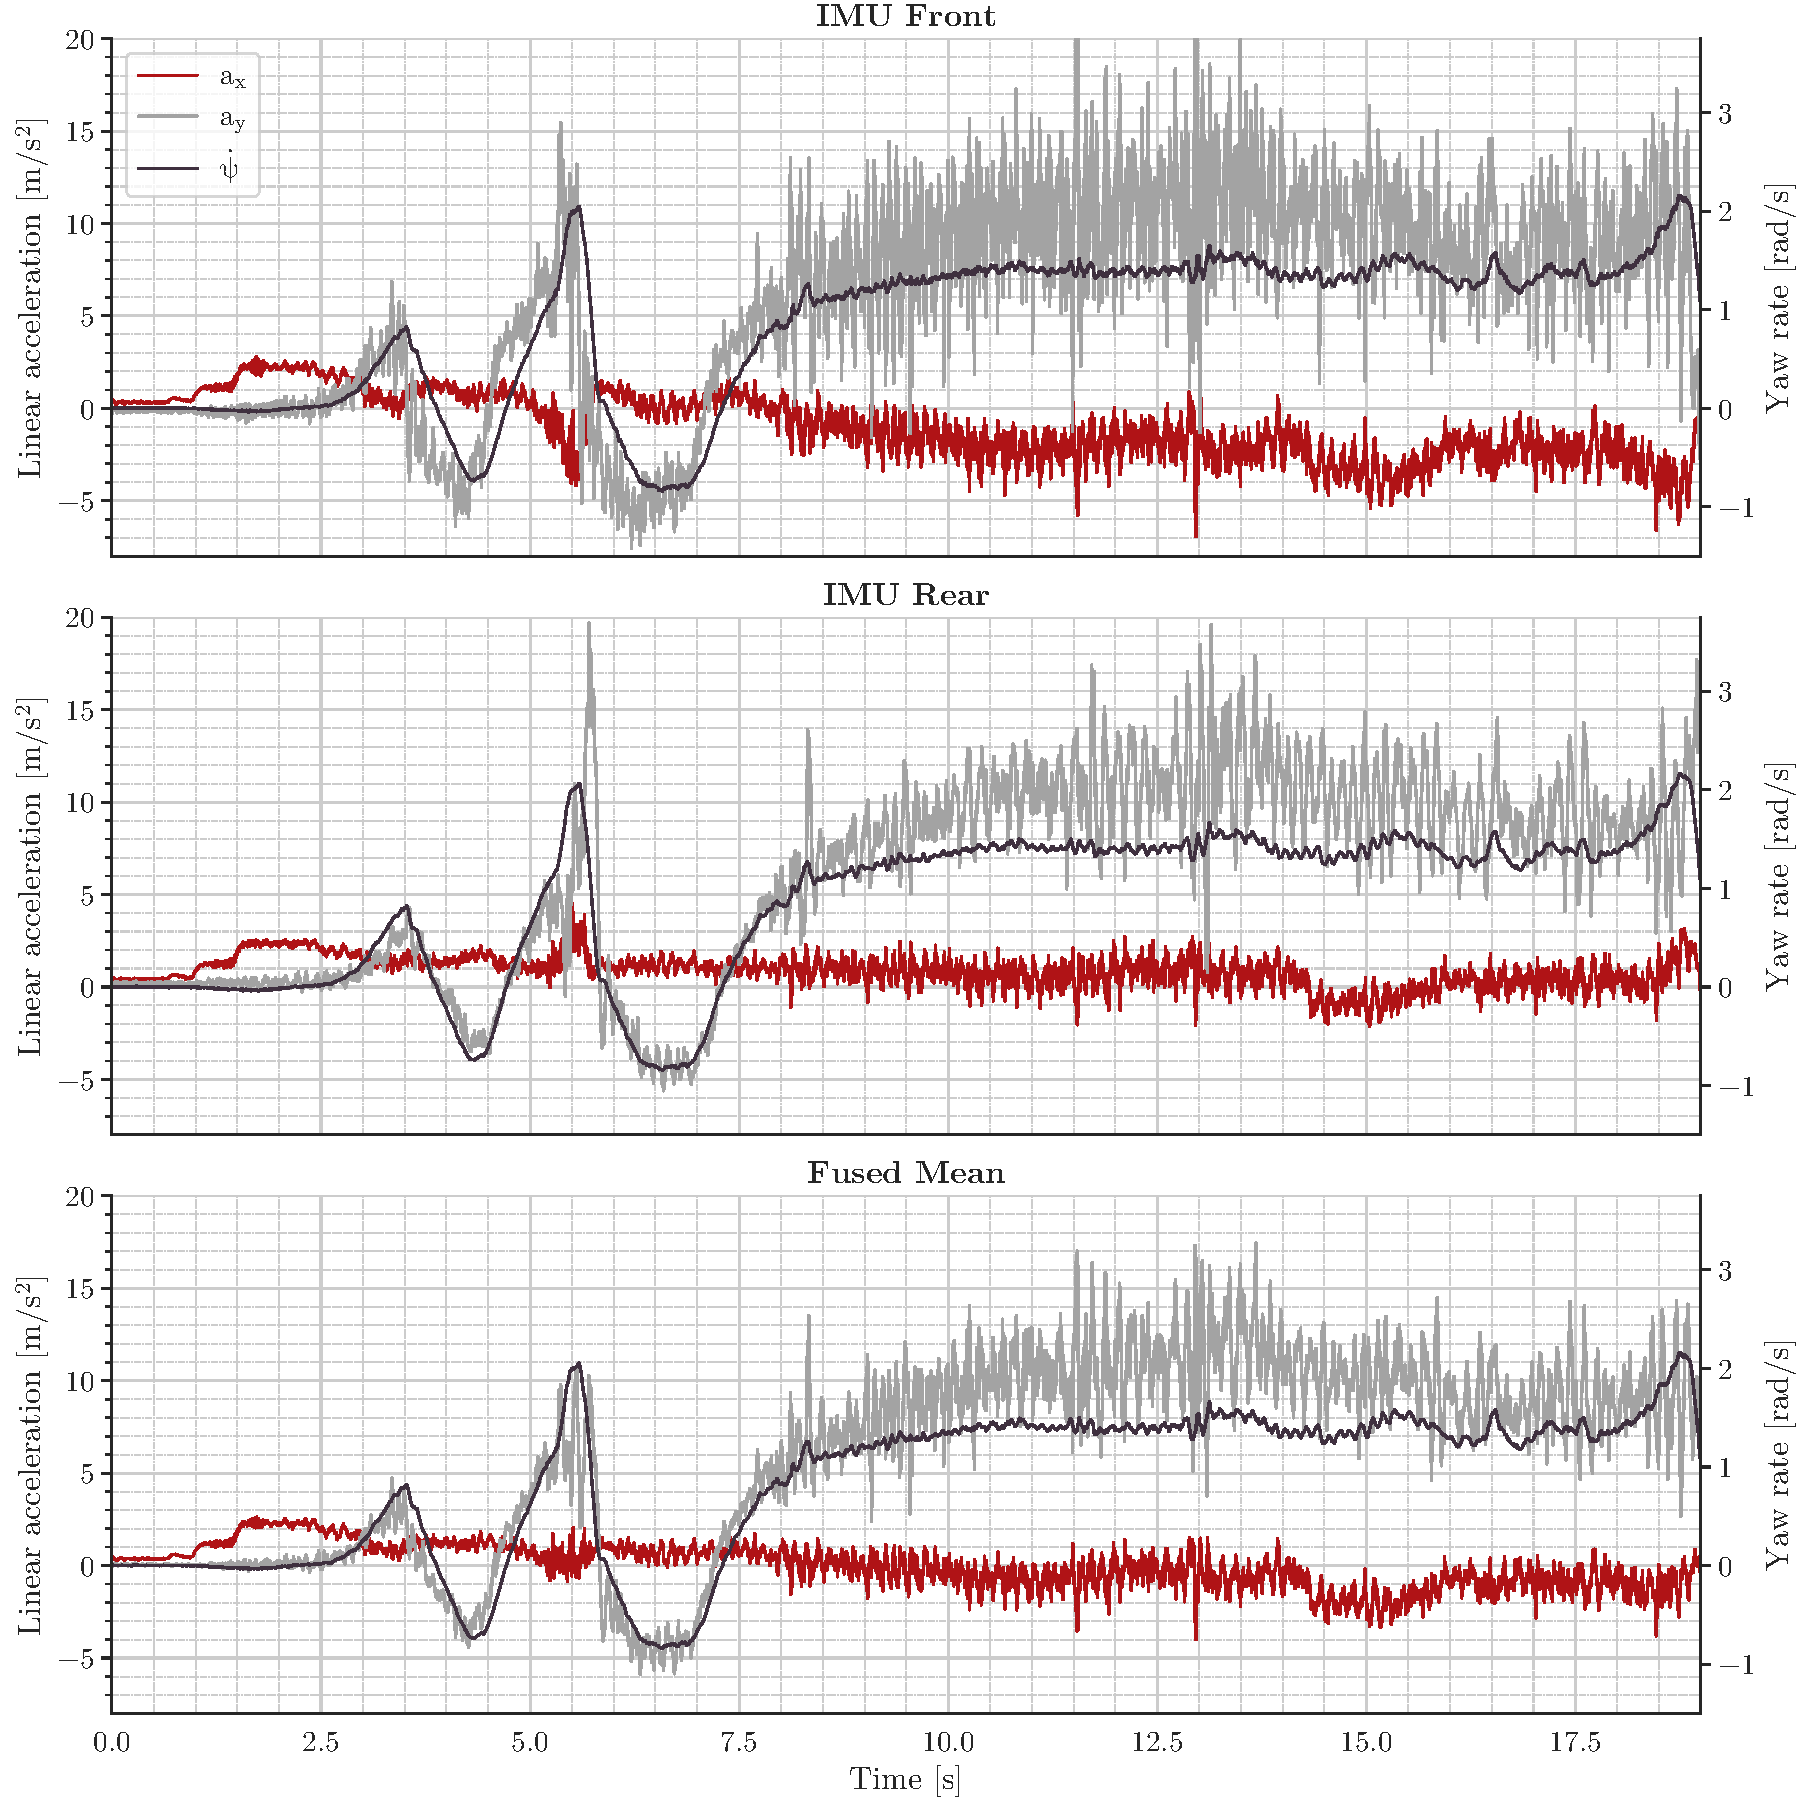
\includegraphics[width=\textwidth]{plot_imu_fusion}%
	\caption{\gls{imu} measurements and fusion results}
	\label{fig:imu-fusion}
\end{figure}


\subsection{Failure Detection}
The effect of the failure detection on the state estimate is shown in figure \ref{fig:failure-detection} for the velocity estimate. The measurement of the optical velocity sensor has a null at around \SI{400}{\milli\second} and two less severe outliers before. The sanity check detects transients through the maximum plausible difference of consecutive samples. It reacts quickly but cannot detect persistent outliers such as the null. The \gls{ekf} bank does not detect the two outliers at the beginning, but excels at detecting the persistent null. Notice how the estimate of much more stable and robust to failures with the failure detection, since the faulty measurements are disabled in the \gls{ekf} and other sensors and the model prediction are used. The stability increases when enabling debouncing with a time of \SI{50}{\milli\second}.

\begin{figure}[t]
	\centering
	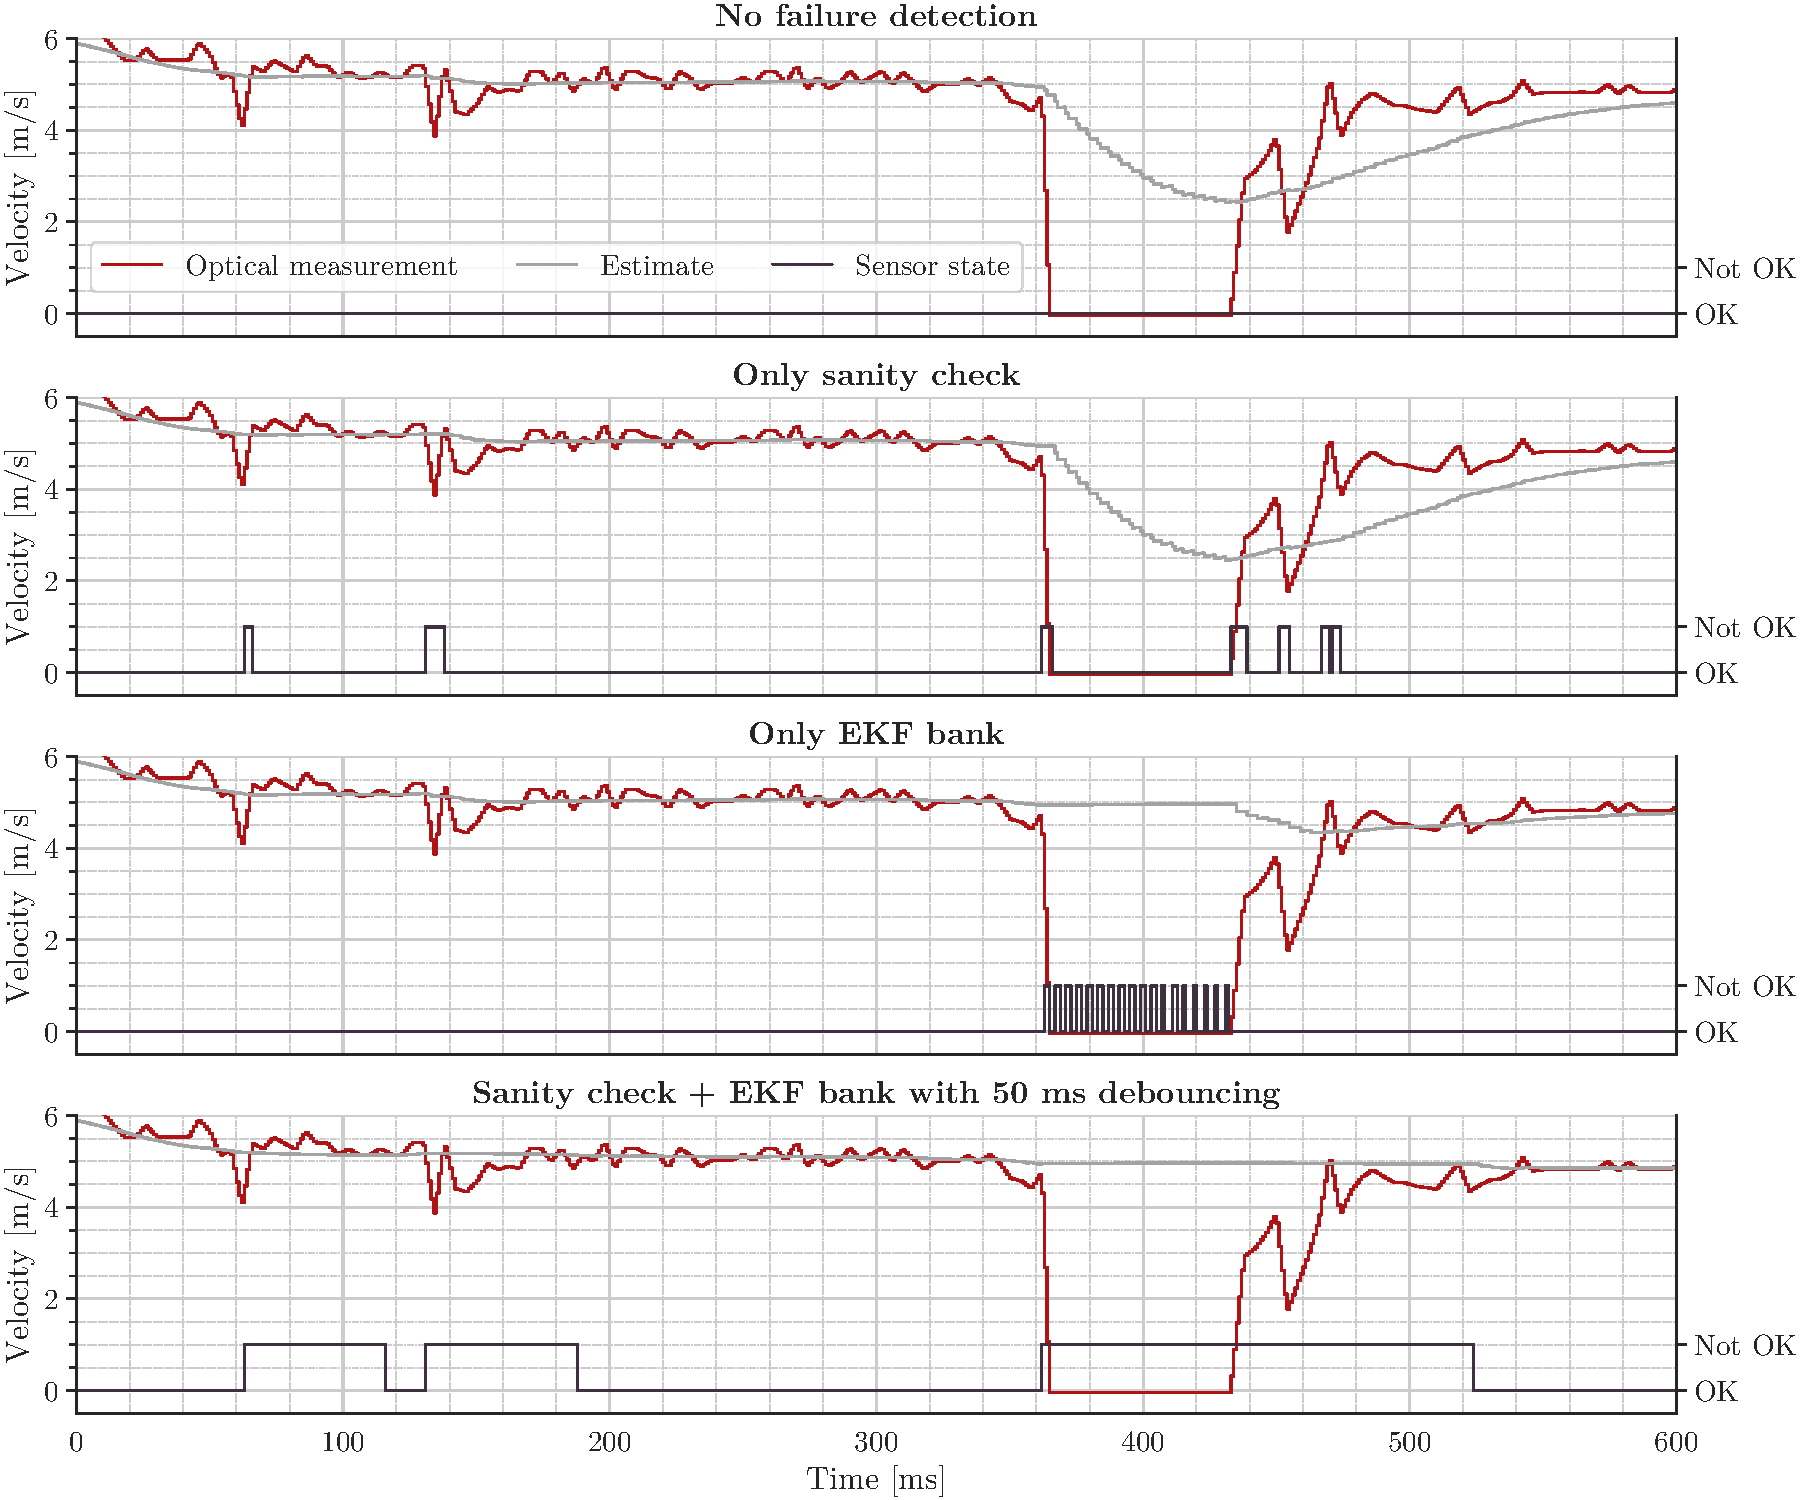
\includegraphics[width=\textwidth]{plot_failure_detection}%
	\caption{Different failure detection modes}
	\label{fig:failure-detection}
\end{figure}

Figure \ref{fig:failure-detection-nssr} shows how large residuals are generated for the \gls{ekf} instances of the bank that do not include the optical sensor. When both residuals cross the threshold, the measurement of the optical sensor is marked as failure. When only one residual crosses the threshold, an outlier cannot be confidently detected. The measurements and residuals of all three velocity sensors for this example can be found in appendix \ref{sec:appendix-failure-detection}. The intermittency of the residuals stems is a result of the difference of \gls{vdc} execution rate and measurement rates.

\begin{figure}[t]
	\centering
	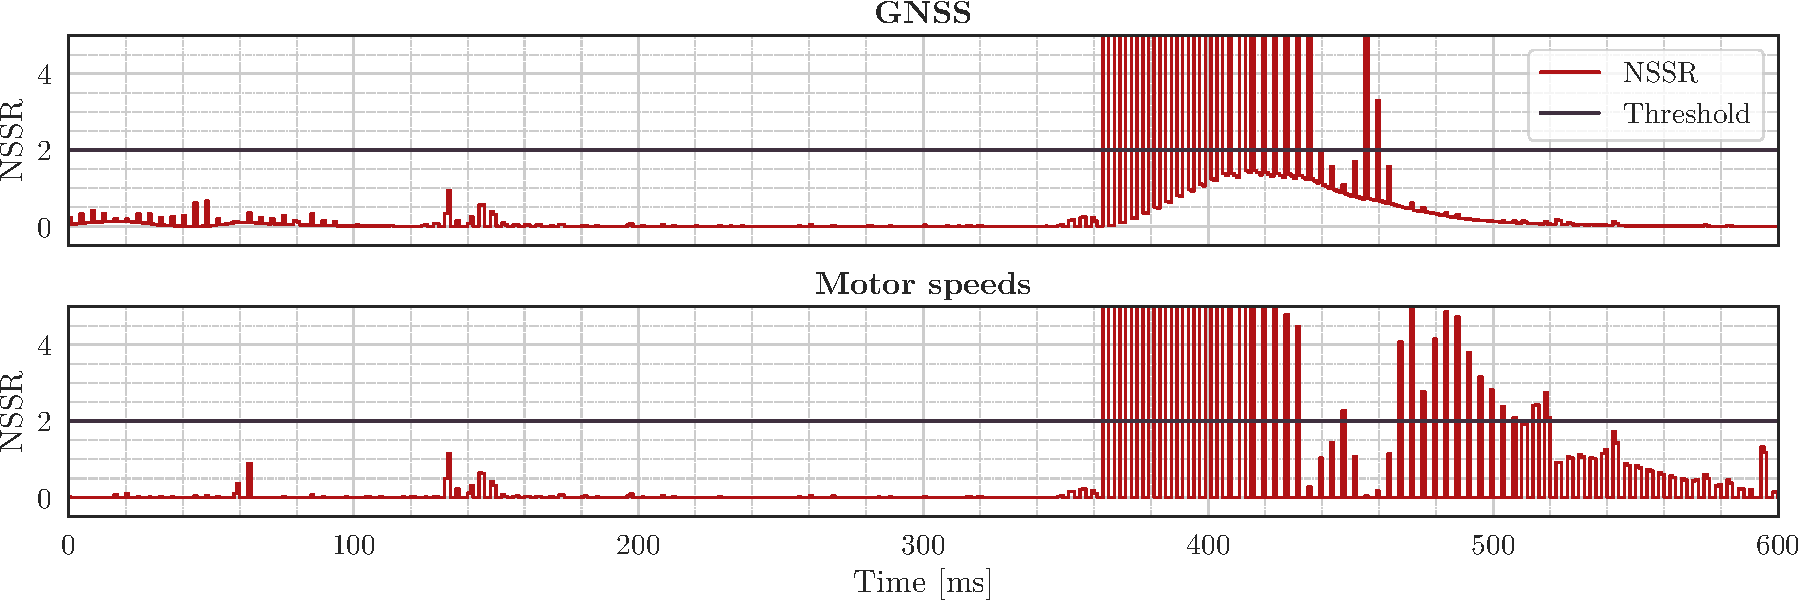
\includegraphics[width=\textwidth]{plot_failure_detection_nssr}%
	\caption{Normalized sums of squared residuals of \gls{ekf} bank}
	\label{fig:failure-detection-nssr}
\end{figure}

The configuration of thresholds and debouncing time has a large impact on failure detection performance. The choice of parameters is always a tradeoff between false positives and false negatives. For example, the \gls{ekf} bank would have recognized the two outliers with a lower threshold, but would be much more prone to noise. Furthermore, a long debouncing time means that a sensor has more time to recover, but that the \gls{ekf} relies only on the model during that time.


\subsection{EKF}
The estimated longitudinal and lateral velocities from the \gls{ekf} are shown in figure \ref{fig:ekf-velocities}. They have much less noise than the sensor measurements and are generally not affected by failures such as spikes in the motor speeds at \SI{5.5}{\second} or the outliers of the optical sensor at \SI{16}{\second}. The residuals for the longitudinal velocity have a mean of zero, which means that predictions match the measurements well, and are low even then the optical sensor is disabled. However, the estimated lateral velocity generally has a lower absolute value than the measurement, which could indicate an inaccurate model. This is especially obvious when disabling the optical sensor, as would be the case in the \gls{dv}.

\begin{figure}[t]
	\centering
	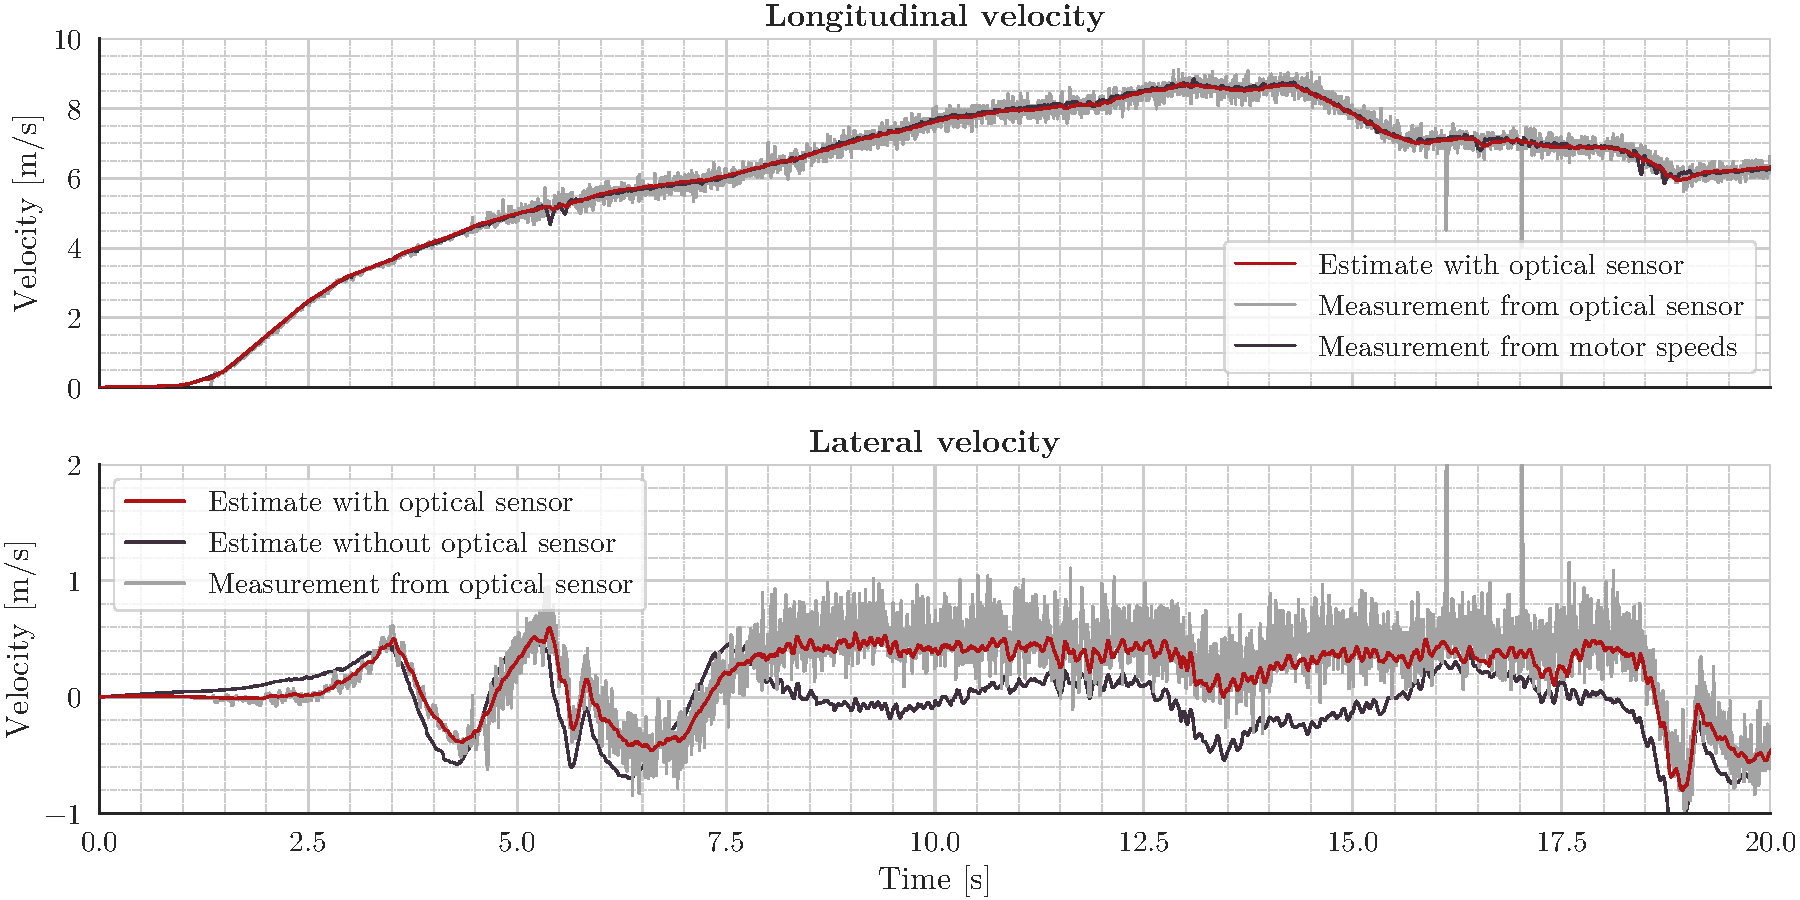
\includegraphics[width=\textwidth]{plot_ekf_velocities}%
	\caption{\gls{ekf} estimate for velocities}
	\label{fig:ekf-velocities}
\end{figure}

The quality of the position estimate depends strongly on the knowledge of the heading, since it related the velocity to the predicted position. Heading measurements are only available in the \gls{dv}, but were not available for evaluation. Therefore we compare the estimates without an initial heading, i.e. $\psi_0 = 0$, and with an initial heading guessed from the vehicle's movement in figure \ref{fig:ekf-position}. The estimate follows the measurement much more closely in the latter case, with lower residuals than when no initial heading is known. The heading itself comes only from the prediction using the yaw rate and is not corrected by measurements. Note that the initial heading is usually not known.
% TODO residuals in appendix
\begin{figure}[t]
	\centering
	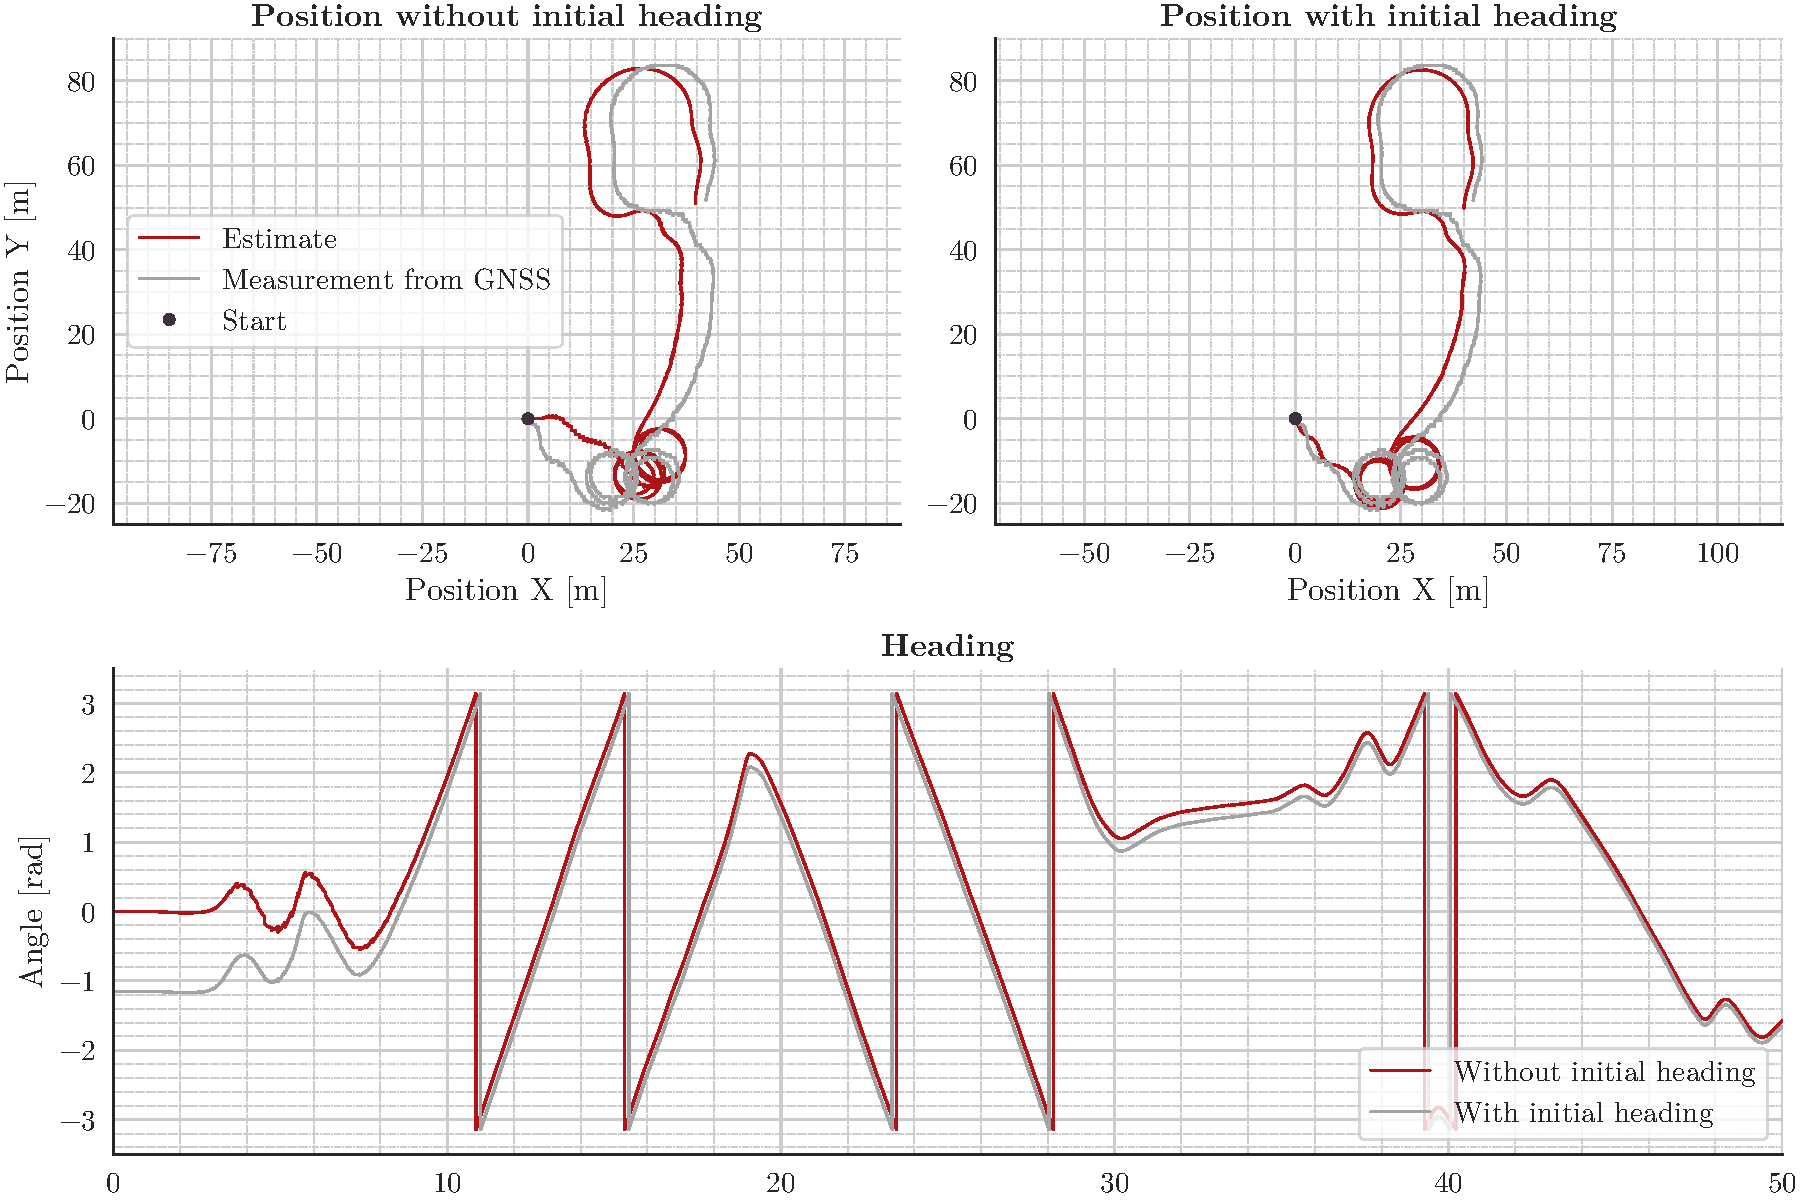
\includegraphics[width=\textwidth]{plot_ekf_pos}%
	\caption{\gls{ekf} estimate for position and heading}
	\label{fig:ekf-position}
\end{figure}

Since the \gls{ekf} estimate is essentially a weighted average, the result varies with the measurement covariance settings. A detailed sensitivity analysis is beyond the scope of this thesis, but in practice, empirically determined settings should be enough.

\section{Discussion}
The results presented in the previous section show, that the state estimation generally works well and improves the quality beyond what raw measurements could provide. The estimate of the longitudinal velocity when the optical sensor is available is especially robust, an important prerequisite for good \gls{tc} performance. The different sensor setups between \gls{ev} and \gls{dv} remain somewhat of a challenge. The evaluation shows that the position estimation only works well with heading measurements, therefore it might be better use raw \gls{gnss} measurements for the \gls{ev}, since a good position estimate is only relevant for the \gls{dv}. Also, the optical velocity sensor is crucial for a good lateral velocity estimate, but a non-linear single track model instead of the kinematic model might mitigate this problem in case the sensor is unavailable.

However, the state estimation needs more extensive testing in real driving situations, on the one hand to calibrate and parametrize the outlier detection and the \gls{ekf}, on the other hand to see if it generalizes well, since the measurement data used for the simulation are not very diverse. Furthermore, they do not include heading measurements and only two \glspl{imu}. With a third \gls{imu}, the maximum-likelihood-based fusion should be revisited, but with two \glspl{imu}, the mean-based fusion is preferable due to its simplicity and less computational complexity. Lastly, other failure detection approaches such as the chi-squared test and variance test can be evaluated in case the present approaches are insufficient.

	\chapter{Conclusion}
	In this thesis, we first presented different approaches for state estimation and failure detection. Then we described the design and implementation of a robust and flexible state estimation for a race car. At the core is a simple three-stage architecture, comprising a preprocessing component for measurement harmonization and \gls{imu} fusion, a unified failure and sensor setup detection providing robustness and support for flexible sensor sets, and an \gls{ekf}-based state estimation performing model-based sensor fusion. Our evaluation shows that the provided state estimate is accurate even in the presence of outliers and sensor failures.

While the estimation of the vehicle velocity is already good, it can likely be improved with a better algorithm for transformation of the motor speeds such as the ones presented in~\cite{Song.2002}. Automated calibration of the \glspl{imu}, i.e. determining the orientation so measurements can be aligned with the vehicle axes, possibly every time the state estimation is started, could be beneficial as well since many components rely on good \gls{imu} measurements. Lastly, a tighter integration with the \gls{dv} software and camera/lidar information could improve state estimation and vehicle performance in the future.

		
	
	\clearpage
	
	%----------------------------------------------------------------------------
	% Appendix
	%----------------------------------------------------------------------------
	
	\cleardoublepage
	\printbibliography

	\printglossary[style=altlist]
	
	\appendix
	\chapter{Expanded Rigid Body Equations}
\section{Transformation of Linear Velocity}\label{sec:appendix-transformation-linvel}
\begin{align*}%
\begin{bmatrix}v_x \\ v_y \\ v_z\end{bmatrix}%
&=\begin{bmatrix}v_{x}^{CG} \\ v_{y}^{CG} \\ v_{z}^{CG}\end{bmatrix}%
+\begin{bmatrix}\dot{\phi} \\ \dot{\theta} \\ \dot{\psi}\end{bmatrix}\times\begin{bmatrix}r_x \\ r_y \\ r_z\end{bmatrix} \\%
&=\begin{bmatrix}v_{x}^{CG} \\ v_{y}^{CG} \\ v_{z}^{CG}\end{bmatrix}%
+\begin{bmatrix}\dot{\theta}r_z - \dot{\psi}r_y \\\dot{\psi}r_x - \dot{\phi}r_z \\\dot{\phi}r_y - \dot{\theta}r_x\end{bmatrix}%
\end{align*}

\section{Transformation of Linear Acceleration}\label{sec:appendix-transformation-linacc}
\begin{align*}%
\begin{bmatrix}a_x \\ a_y \\ a_z\end{bmatrix}%
&=\begin{bmatrix}a_{x}^{CG} \\ a_{y}^{CG} \\ a_{z}^{CG}\end{bmatrix}%
+\begin{bmatrix}\ddot{\phi} \\ \ddot{\theta} \\ \ddot{\psi}\end{bmatrix}\times\begin{bmatrix}r_x \\ r_y \\ r_z\end{bmatrix}%
+\begin{bmatrix}\dot{\phi} \\ \dot{\theta} \\ \dot{\psi}\end{bmatrix}\times \left(\begin{bmatrix}\dot{\phi} \\ \dot{\theta} \\ \dot{\psi}\end{bmatrix}\times\begin{bmatrix}r_x \\ r_y \\ r_z\end{bmatrix}\right)\\%
&=\begin{bmatrix}a_{x}^{CG} \\ a_{y}^{CG} \\ a_{z}^{CG}\end{bmatrix}%
+\begin{bmatrix}\ddot{\phi} \\ \ddot{\theta} \\ \ddot{\psi}\end{bmatrix}\times\begin{bmatrix}r_x \\ r_y \\ r_z\end{bmatrix}%
+\begin{bmatrix}\dot{\phi} \\ \dot{\theta} \\ \dot{\psi}\end{bmatrix}\times\begin{bmatrix}\dot{\theta}r_z - \dot{\psi}r_y \\\dot{\psi}r_x - \dot{\phi}r_z \\\dot{\phi}r_y - \dot{\theta}r_x\end{bmatrix}\\%
&=\begin{bmatrix}a_{x}^{CG} \\ a_{y}^{CG} \\ a_{z}^{CG}\end{bmatrix}%
+\begin{bmatrix}\ddot{\theta}r_z - \ddot{\psi}r_y \\\ddot{\psi}r_x - \ddot{\phi}r_z \\\ddot{\phi}r_y - \ddot{\theta}r_x\end{bmatrix}%
+\begin{bmatrix}\dot{\theta}(\dot{\phi}r_y - \dot{\theta}r_x) - \dot{\psi}(\dot{\psi}r_x - \dot{\phi}r_z)\\\dot{\psi}(\dot{\theta}r_z - \dot{\psi}r_y) - \dot{\phi}(\dot{\phi}r_y - \dot{\theta}r_x)\\\dot{\phi}(\dot{\psi}r_x - \dot{\phi}r_z) - \dot{\theta}(\dot{\theta}r_z - \dot{\psi}r_y)\end{bmatrix}%
\end{align*}

\chapter{Extended Kalman Filter Equations}\label{sec:appendix-ekf-equations}

\section{Jacobian of Process Function With Respect to State Vector}
\begin{equation*}%
\frac{\partial \dot{x}}{\partial x} = \begin{bmatrix}%
0 & 0 & cos(\psi) & -sin(\psi) & -v_x \cdot sin(\psi) - v_y \cdot cos(\psi) & 0 \\%
0 & 0 & sin(\psi) & cos(\psi) & v_x \cdot cos(\psi) - v_y \cdot sin(\psi) & 0 \\%
0 & 0 & 0 & \dot{\psi} & 0 & v_y \\%
0 & 0 & -\dot{\psi} & 0 & 0 & -v_x \\%
0 & 0 & 0 & 0 & 0 & 1 \\%
0 & 0 & 0 & 0 & 0 & 0%
\end{bmatrix}%
\end{equation*}

\section{Jacobian of Process Function With Respect to Input Vector}
\begin{equation*}%
\frac{\partial \dot{x}}{\partial u} = \begin{bmatrix}%
0 & 0 & 0 \\%
0 & 0 & 0 \\%
1 & 0 & 0 \\%
0 & 1 & 0 \\%
0 & 0 & 0 \\%
0 & 0 & 1%
\end{bmatrix}%
\end{equation*}

\section{Measurement Matrix}\label{sec:appendix-ekf-measurement}
\begin{equation*}%
H = \begin{bmatrix}%
1 & 0 & 0 & 0 & 0 & 0 \\%
0 & 1 & 0 & 0 & 0 & 0 \\%
0 & 0 & 1 & 0 & 0 & 0 \\%
0 & 0 & 0 & 1 & 0 & 0 \\%
0 & 0 & 1 & 0 & 0 & 0 \\%
0 & 0 & 1 & 0 & 0 & 0 \\%
0 & 0 & 0 & 0 & 1 & 0 \\%
0 & 0 & 0 & 0 & 0 & 1%
\end{bmatrix}%
\end{equation*}

\end{document}